 \section{Vectors}
Imagine an arrow, floating in space. Try to describe where in space it is to someone else. It's difficult, isn't it?
Now, imagine that same arrow on the Cartesian plane, with its tail on the origin. Describe where the arrow is by giving the coordinates of the tip of the arrow, in the form $\begin{bmatrix}x\\y\end{bmatrix}$.
Much easier, right? Well, we call these arrows vectors, and they represent both magnitude (the length of the vector) and direction (which way the vector is pointing). 
\begin{figure}[H]
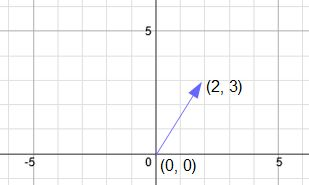
\includegraphics{visualvectordotproduct1.jpg}
\end{figure}
In the figure above, you'll see how we look at vectors. The vector is represented by the coordinates of the tip of the vector, with the tail on the origin. We can perform operations on vectors, like adding. A diagram of this is shown below.
\begin{figure}[H]
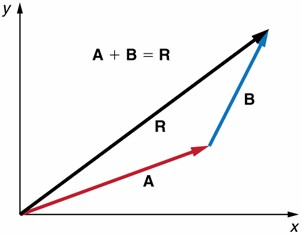
\includegraphics{Figure_03_03_05a.jpg}
\end{figure}
Geometrically, adding is done by placing the second vector's tail at the tip of the first vector, and drawing the new vector from the tail of the first to the tip of the second. Mathematically, this is done by doing $\begin{bmatrix}x_1\\y_1\end{bmatrix}+\begin{bmatrix}x_2\\y_2\end{bmatrix}=\begin{bmatrix}x_1+x_2\\y_1+y_2\end{bmatrix}$. So adding vectors is fairly simple, and subtraction of vectors operates on the same principle.
We can also multiply vectors by normal numbers, or scalars. 
\begin{figure}[H]
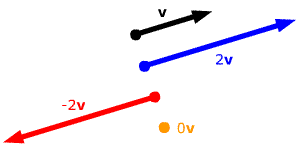
\includegraphics{mult2.png}
\end{figure}
The scalar stretches the vector if it is positive and greater than one, keeps the vector the same if it is one, shrinks the vector while less than one and greater than zero, makes the vector into a point if it is zero, and flips the vector and stretches or shrinks it as described if it is negative.
In this, it is just like multiplication of two normal numbers. The next important thing about vectors is that there are basis vectors. Imagine a small vector, taking up one unit of each of the axes on the coordinate plane. 
\begin{figure}[H]
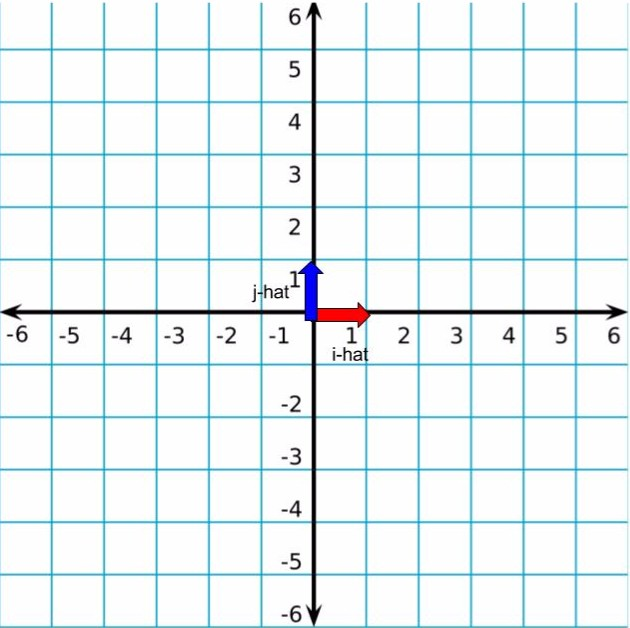
\includegraphics{basis.jpg}
\end{figure}
These two vectors are called $\hat{i}$ (read i-hat) and $\hat{j}$ (read j-hat). What's interesting is that all vectors are composed of these basis vectors (a new basis vector is added for each dimension). How? Well, let's say we have a vector $\mathbb{v}$ (variables for vectors are commonly bolded or written with an arrow on top). We can write it as a scalar $a$ multiplied by the basis vector $\hat{i}$ plus another scalar $b$ multiplied by the basis vector $\hat{j}$. You can also pick different basis vectors, by changing the axes, and get a new logical system.
\section{Matrices}
So we have this concept of vectors. But linear algebra isn't just about vectors, it also talks about matrices. Basically, matrices represent transformations of the coordinate plane, and all the vectors in it. A transformation is a function, with vector inputs and outputs. The functions, however, must be linear. This can be thought of geometrically as keeping all of the gridlines of the coordinate plane straight and parallel, and keeping them from getting curved. The other rule is that the origin must remain fixed in place.
So, how do matrices represent this transformation? Well, they just show where $\hat{i}$ and $\hat{j}$ end up. So, if $\hat{i}$'s coordinates are $\begin{bmatrix}\hat{i}_x\\\hat{i}_y\end{bmatrix}$ and $\hat{j}$'s coordinates are $\begin{bmatrix}\hat{j}_x\\\hat{j}_y\end{bmatrix}$, the matrix representing that transformation would be $\begin{bmatrix}\hat{i}_x & \hat{j}_x\\\hat{i}_y & \hat{j}_y\end{bmatrix}$. We can multiply this matrix by any vector to get what the coordinates of that vector would be in the new system.
Suppose, however, that we wish to do two transformations. Instead of applying each matrix separately, we can multiply the two matrices and apply that new matrix to the vector. Suppose we have two matrices, how do we multiply them? We can do
\begin{equation*}
\begin{bmatrix}a&b\\c&d\end{bmatrix}\begin{bmatrix}e&f\\g&h\end{bmatrix}=\begin{bmatrix}ae+bg&af+bh\\ce+dg&cf+dh\end{bmatrix}
\end{equation*}
\section{Determinants}
The next important thing about linear algebra is the determinant. Basically, the deteriminant is the area of one grid square.
\begin{figure}[H]
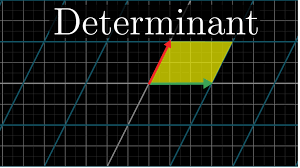
\includegraphics{determinant.png}
\end{figure}
The determinant changes depending on the basis vectors. Because a matrix represents a linear transformation, and therefore the basis vectors, we can calculate the determinant of a 2x2 matrix as follows:
\begin{equation*}
\det\left(\begin{bmatrix}a&b\\c&d\end{bmatrix}\right)=ad-bc
\end{equation*}
Calculating the determinant is different if you have a 3x3 matrix (remember that the size of a matrix represents the number of dimensions the transformation is taking place in).
\section{Dot Product}
A dot product is a simple function that takes in two vectors and outputs a scalar as follows:
\begin{equation*}
\begin{bmatrix}a\\b\end{bmatrix}\begin{bmatrix}c\\d\end{bmatrix}=ac+bd
\end{equation*}
It will be useful later on in these notes.
\section{Solving Systems of Equations}
One of the many useful applications of linear algebra is solving systems of equations. For example, let's say we have the system of equations $2x+2y=-4$ and $x+3y=-1$. We can solve this by putting all the coefficients in a matrix, all the variables in a vector, and all the constants in a vector:
\begin{equation*}
\begin{bmatrix}2&2\\1&3\end{bmatrix}\begin{bmatrix}x\\y\end{bmatrix}=\begin{bmatrix}-4\\-1\end{bmatrix}
\end{equation*}
We can solve this by multiplying each side by the inverse of the matrix. This makes sense - if we are solving a simpler equation, say $5x=10$, we solve by dividing each side by $5$, because division is the inverse of multiplication. The inverse of the matrix is a matrix that, when multipled by the original matrix, produces the identity matrix. The identity matrix is kind of like $1$ - when applied to other matrices, it doesn't change anything. The identity matrix is $\begin{bmatrix}1&0\\0&1\end{bmatrix}$. You can test it for yourself. To find the inverse of a 2x2 matrix, we can follow the following rule (where $A$ is the original matrix, and $A = \begin{bmatrix}a&b\\c&d\end{bmatrix}$):
\begin{equation*}
\frac{1}{\det(A)}\begin{bmatrix}d&-b\\-c&a\end{bmatrix}
\end{equation*}
The rule is different, and more complicated, for 3x3 matrices. In the case of our system of equations from earlier, the inverse is $\begin{bmatrix}\frac{3}{4}&-\frac{1}{2}\\-\frac{1}{4}&\frac{1}{2}\end{bmatrix}$. Multiplying it by both sides produces the equation
\begin{equation*}
\begin{bmatrix}x\\y\end{bmatrix}=\begin{bmatrix}-\frac{11}{4}\\-\frac{5}{2}\end{bmatrix}
\end{equation*}
And so we have the solutions to our system.
